For this part, let's explore how we designed the board, from the schematic
to a working PCB layout !

% Schematic
First, we're going to dig into the schematic we've done for the physical part
of controller. Thus, we're going to start with a global schematic part, where
we explain the organization of the pages, and then we'll dig a bit deeper into
the differents blocs.

The whole schematic is available at the end of this report, in the annexes
\ref{annex:schematic}.

\section{Power supplies}
Now, let's look a bit deeper on the power supplies, and how they're agenced.
\subsection{Power tree}
To represent the whole power supply organization, we drew a power tree, a schematic that
represent the power supplies.

\begin{figure}[!ht]
    \centering
    \resizebox{\SchematicWidth}{!}{%
        \begin{circuitikz}
            \tikzstyle{every node}=[font=\large]
            \draw [ fill={rgb,255:red,195; green,232; blue,235} ] (-1.25,17.25) rectangle  node {\large Battery 1} (3.75,14.75);
            \draw [ fill={rgb,255:red,195; green,232; blue,235} ] (-1.25,11) rectangle  node {\large Battery 2} (3.75,8.5);
            \draw [ fill={rgb,255:red,218; green,187; blue,217} ] (-1.25,4.75) rectangle  node {\large USB} (3.75,2.25);
            \draw [ fill={rgb,255:red,233; green,235; blue,199} ] (8.75,17.25) rectangle  node {\normalsize 5V buck (2A)} (13.75,14.75);
            \draw [ fill={rgb,255:red,233; green,235; blue,199} ] (8.75,11) rectangle  node {\large 3.3V Buck (200 mA)} (13.75,8.5);
            \draw [ fill={rgb,255:red,236; green,195; blue,195} ] (18.75,17.25) rectangle  node {\large Servo and power circuits} (23.75,14.75);
            \draw [ fill={rgb,255:red,158; green,148; blue,213} ] (18.75,11) rectangle  node {\large Logic IC and analog circuits} (23.75,8.5);
            \draw (6.25,4.75) to[D] (6.25,8.5);
            \draw [short] (3.75,3.5) -- (6.25,3.5);
            \draw [short] (6.25,4.75) -- (6.25,3.5);
            \draw [short] (3.75,9.75) -- (8.75,9.75);
            \draw [short] (6.25,8.5) -- (6.25,9.75);
            \draw [short] (3.75,16) -- (8.75,16);
            \draw [short] (13.75,16) -- (18.75,16);
            \draw [short] (13.75,9.75) -- (18.75,9.75);
            \draw [dashed] (6.25,9.75) -- (6.25,16);
            \node [font=\large] at (5,16.5) {7.4V - 8.2V};
            \node [font=\large] at (5,10.25) {4.3V - 8.2V};
            \node [font=\large] at (15.25,16.5) {5V};
            \node [font=\large] at (15.25,10.25) {3.3V};
            \draw [dashed] (6.25,16) -- (6.25,18.5);
            \draw [dashed] (6.25,18.5) -- (16.25,18.5);
            \draw [dashed] (16.25,18.5) -- (16.25,16);
        \end{circuitikz}
    }%
    \label{fig:power_tree}
    \caption{}
\end{figure}
\FloatBarrier

On this schematic, there two main regulators, that are, in fact buck switching regulators.
But, there's three power sources :
\begin{itemize}[noitemsep]
    \item   Vbus : The 5V that came from the USBC port when the board is plugged on a PC.
    \item   Vbatt : A battery that is charged to power up the MCU and all of the logic
          circuits.
    \item   Vbatt\_pyro : A battery that is charged to power up the servo engines and
          the thruster starter.
\end{itemize}.

As we can see in \ref{fig:power_tree}, we can configure the power supply as we need.
From the three sources, we're able to use a single one by tying both supply together.
And, we can even then supply the whole system with a single USB supply, but at a reduced
voltage. At the opposite, if needed, we can bypass the 5V buck system if we want to
power the servos and the engines with an higher voltage.

Selection is mainly done by jumper, which are big zero ohm resistors.

\subsection{DCDC buck design}
To design theses circuits, we used a reliable tool that may be found online, from
Texas Instruments : \cite{POWERDESIGNER}. We pass them the input conditions, such as
voltage, and the output wanted : voltage and current. The tool output then circuits
than can match the needs, and we need to select one, based on some settings :

\begin{itemize}[noitemsep]
    \item   Space on board
    \item   Cost
    \item   switching frequency
\end{itemize}

Since we didn't require specific criterion on theses aspects, we choose the one that
was the easiest to solder. Then, we import the designed module into the schematic.

\section{Digital part}
For this second part, the digital one we're going to look at the
microcontroller mostly, but also some parts of the whole digital subsystems.
For this part, we mostly got inspired by development kits, such as
\cite{nRF5340DK}. These provide a great example on how to implement some IC on
custom PCBs.

Around the MCU, we added some peripherals IC to fulfill our needs, for examples
:
\begin{itemize}[noitemsep]
    \item An 16 Mb EEPROM, to store flight measurements.
    \item An RGB LED, to indicate status to the user.
\end{itemize}

To ensure the systems are working we sometimes need to modify some elements
from the examples. These changes are always documented in the datsheets of the
components.

Here some examples of things we changed :
\begin{itemize}[noitemsep]
    \item   Change configuration bootstrap to select one mode of the other.
    \item   Configure power supplies needed.
    \item   Configure I2C addresses.
\end{itemize}

\subsection{Pin attribution}
To understand how we assigned to each functions some pins on the MCU, we need
to read the datasheets, mainly the MCU one. It's clearly explained that any
peripheral can be routed to any pins a pin matrix . Nonetheless, there's some
pins that can designed for a specific function. For example, there is two pins
designed for high drain current, where the opposite direction (pull up) is
standard. These pins are designed to handle high speed I2C ! So if we want to
use fast I2C, it's clearly recommended to use them.

The remaining pins were placed arbitrary, because we'll changed that later !
\ref{sec:pin_swap}.

\subsection{Discrete logic}\label{subsec:dis_logic}
On the board, most of the logic is done in software by the MCU. But there's two
hardware functions, related to security features.

These are latching the state of the pin with a DLATCH on the boot of the board,
and an AND gate between the command of the engines and input of the drivers.

This enable us to block the start of engines in hardware rather than by
software only. Thus, if the board is configured as debug mode, it won't be able
to start engines, regardless of the software loaded.

\section{Analog conception}
Now, let's jump into the analog design we've done : 
The analog is quite absent on this board, and we only use it for two purposes :

\begin{itemize}[noitemsep]
    \item   Get the position feedback of the servos.
    \item   Monitor voltages on power rails. 
\end{itemize}

For this part, we're measuring a DC voltage that move between $~0.6 \si{\volt}$
and $~2.4 \si{\volt}$. And, they're moving slowly, it take near one second to get
from one limit to the other ! For the second part, we're measuring a static DC voltage,
just to ensure the battery is present and in it's operating range.

Since the voltages are already in our measurement range, and even more, in the area
where the integrated ADC is quite linear, we don't have a lot of signal conditioning
to do.

We've only designed a filter to remove any high frequency signals that may be picked
by the wires used. Thus, we designed a Sallen-Key active filter, with a 100 Hz cutoff
frequency. This filter is absent from the power supply rail measurements, since they
are located on the PCB, and we can ensure the signal integrity with a proper layout.

The circuit is the following one :
\begin{figure}[!ht]
    \centering
    \resizebox{\SchematicWidth}{!}{%
        \begin{circuitikz}
            \tikzstyle{every node}=[font=\normalsize]
            \draw (5,12.25) to[european resistor,l={ \normalsize R1 = 16k$\Omega$}] (7.5,12.25);
            \draw (8.75,12.25) to[european resistor,l={ \normalsize R2 = 16k$\Omega$}] (11.25,12.25);
            \draw (15.25,12.75) node[op amp,scale=1] (opamp2) {};
            \draw (opamp2.+) to[short] (13.75,12.25);
            \draw  (opamp2.-) to[short] (13.75,13.25);
            \draw (16.45,12.75) to[short](16.75,12.75);
            \draw (12.5,12.25) to[C,l={ \normalsize C1 = 100nF}] (12.5,9.75);
            \draw (8.75,14.75) to[C,l={ \normalsize C2 = 100nF}] (11.25,14.75);
            \draw (7.5,12.25) to[short] (8.75,12.25);
            \draw (11.25,12.25) to[short] (13.75,12.25);
            \draw (8.75,14.75) to[short] (8,14.75);
            \draw (8,14.75) to[short] (8,12.25);
            \draw (11.25,14.75) to[short] (17.5,14.75);
            \draw (17.5,14.75) to[short] (17.5,12.75);
            \draw (16.75,12.75) to[short] (17.5,12.75);
            \draw (13.75,13.25) to[short] (12.5,13.25);
            \draw (12.5,13.25) to[short] (12.5,14.75);
            \node at (12.5,12.25) [circ] {};
            \node at (12.5,14.75) [circ] {};
            \draw (5,12.25) to[short, -o] (3.75,12.25) node[left] {Vin};
            \draw (17.5,12.75) to[short, -o] (18.75,12.75) node[right] {Vout};
            \draw (12.5,9.75) to (12.5,9.5) node[ground]{};
        \end{circuitikz}
    }%
    \caption{Circuit for the filter}\label{fig:servo-filter}
\end{figure}
\FloatBarrier

Using a SPICE simulator, we got this response :
\begin{figure}[!hbt]
    \centering
    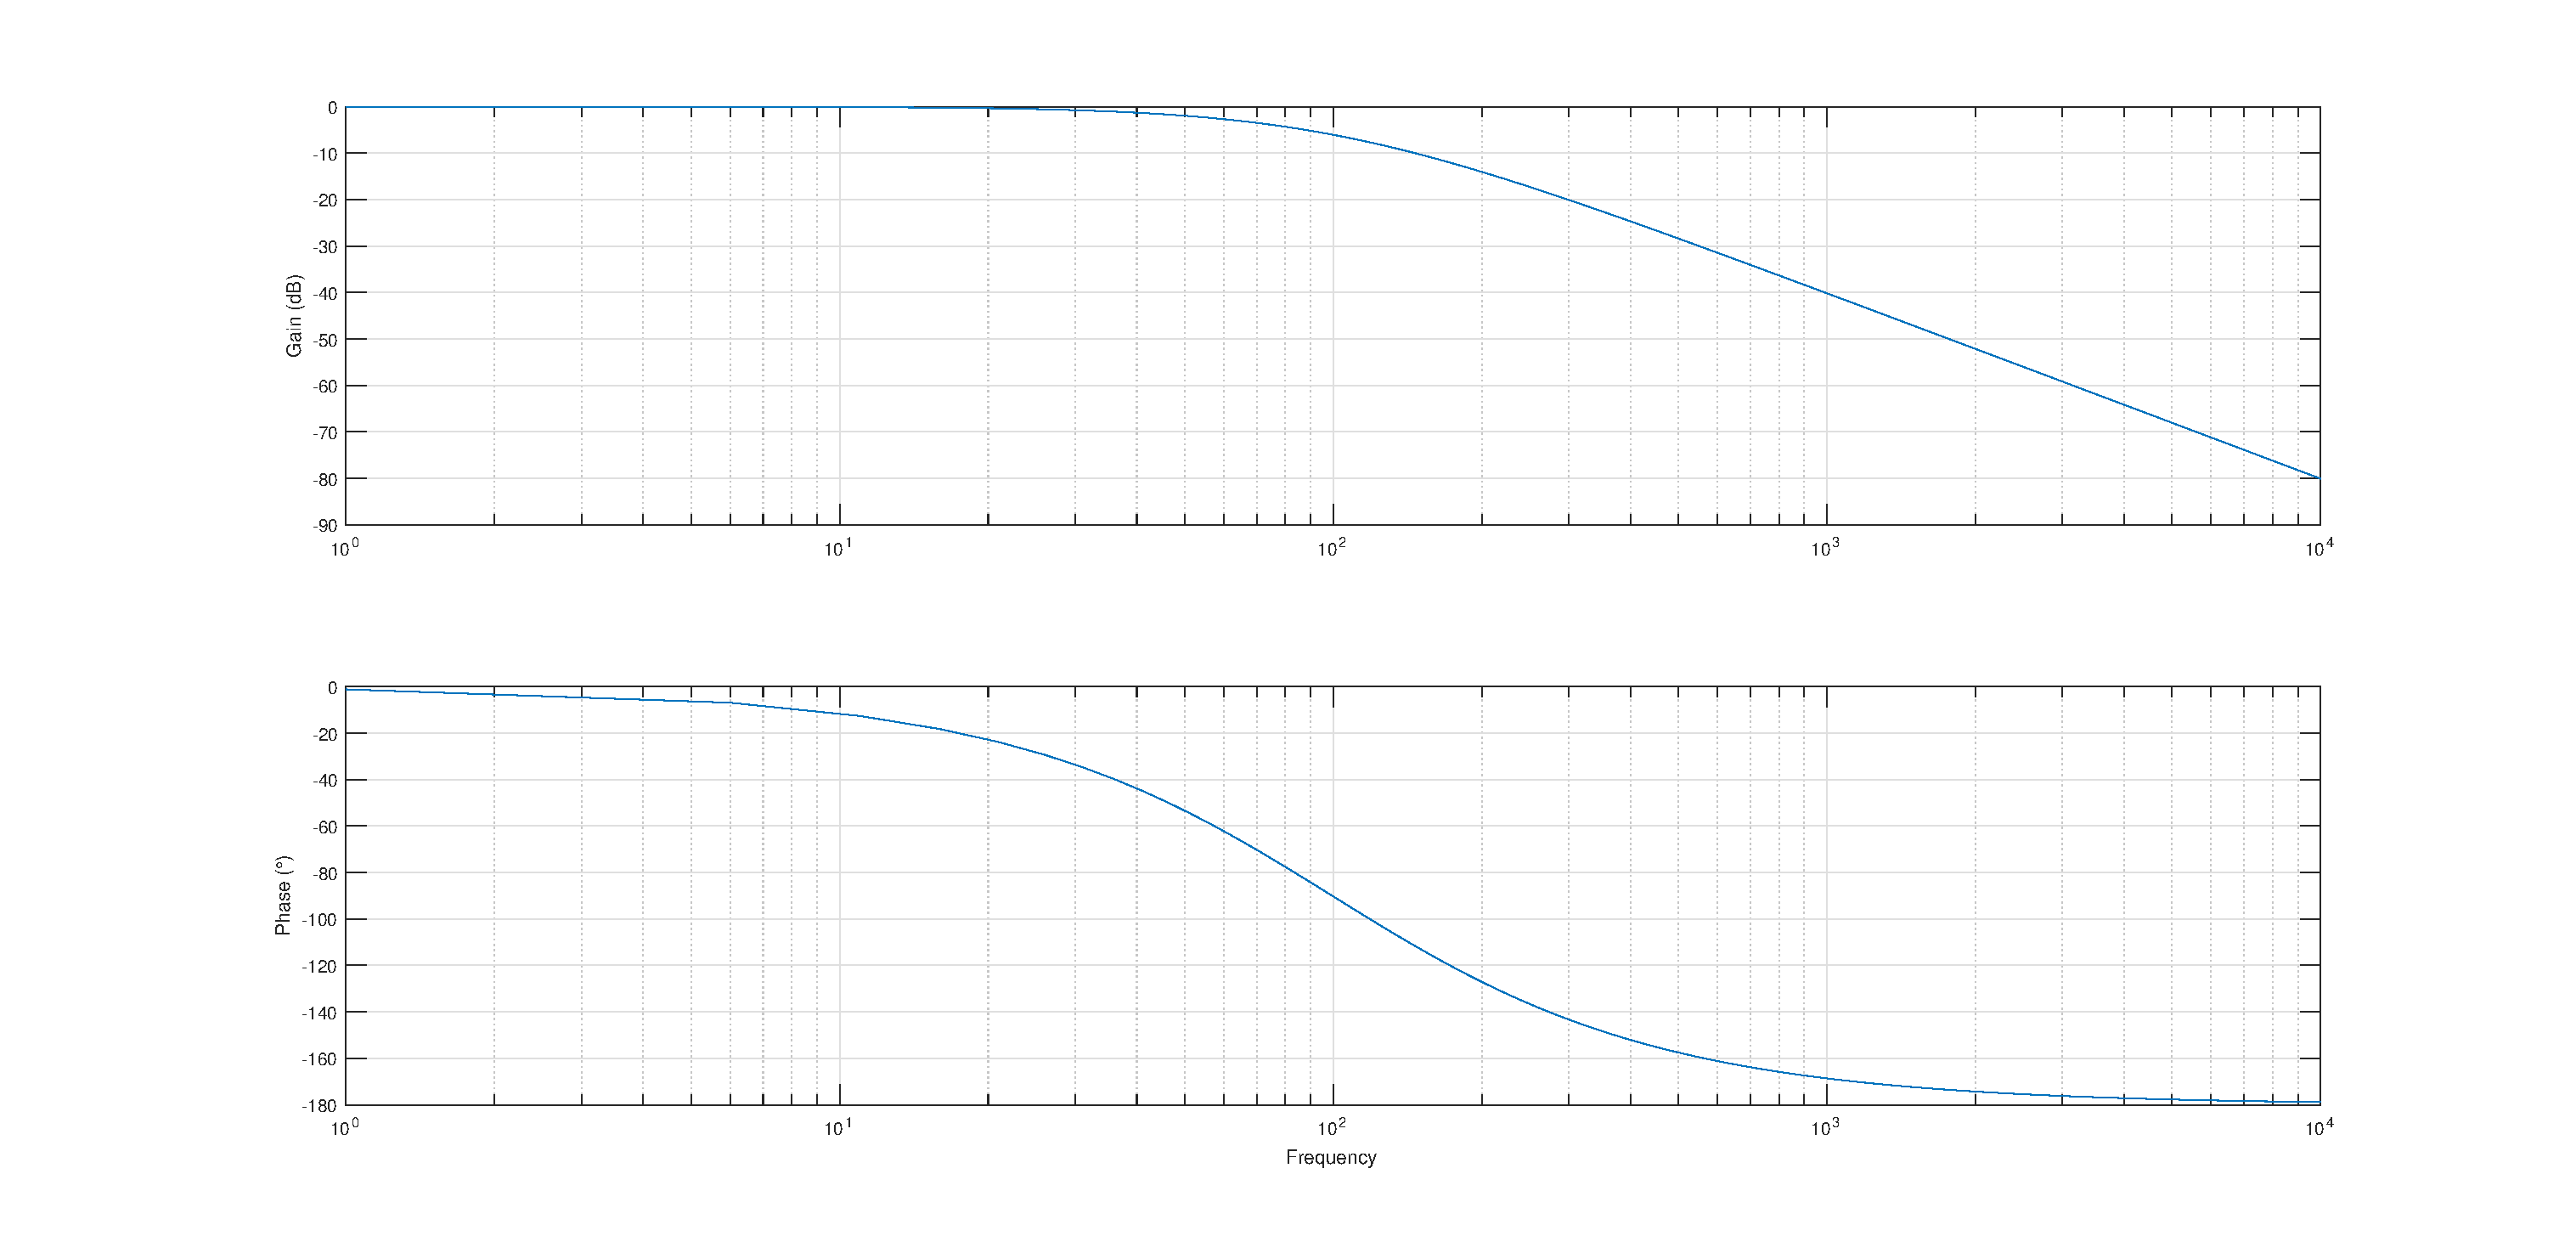
\includegraphics[width=\SchematicWidth]{\Images/Schematic/filter.eps}
    \caption{Bode plot of the filter response}
\end{figure}
\FloatBarrier

The response match our needs, which are quite simple : Remove the potential harmfull noise,
and fast variations that could occur. 

The real circuit on the schematic is based on this one, but with optionnal configurations
jumpers to enable to tune the circuit on board.

This include : 
\begin{itemize}[noitemsep]
    \item   An optionnal voltage divider at the input, to not go above the rail of the OpAmp.
    \item   Optionnals jumpers to bypass the frontend directly to the ADC.
\end{itemize}
\section{Power section}
Now, let's look into the power section of the board. This is this section
responsible to power up the heaviest devices, which can't be powered from a
GPIO.

There's few devices on the board that require specific circuits to be driven :

\begin{itemize}[noitemsep]
    \item   The servomotors (ailerons and parachute).
    \item   The buzzer.
    \item   The engine starters.
\end{itemize}

Each of these elements go it's solution since they're requirements aren't the
same.

\subsection{Servomotors}
These devices are already an integrated solution, we don't directly drive the
servo. So, their power requirements are quite easy to fulfill : We feed them
with 5V, stable voltage.

We only used bulk capacitors near their connectors to ensure that a current
peak is handled it locally.

\subsection{Buzzer}
This second device is a different beast, since we drive it directly. This time,
we placed it directly on the supply, with an NMOS on the low side, to switch on
or off the current on it, and thus make sound, or not.

So, we needed an NMOS transistor to be choosen that can handle some current,
but more importantly : An NMOS that was compatible with our voltage level
available on the output of GPIOs\footnote{ The mosfet we choosed was working,
    the can be optimized : We didn't make sure that is was fully switched at our
    GPIO voltage level, and thats effectively the case : It fully switch at arround
    6V. Thus, the current is limited, which is fine for logic usages but not power
    ones. }.

\subsection{Engine starters}
For these last one, this is where our requirements are the highest : We need a
lot of current, around 2A per engine to start, at a quite high voltage (8-9V).

The power supply for this section is different than the remaining of the board,
for a simple reason : When the engine start, the supply is near the short
circuit. It's voltage will then drop, and it may place others components in
UVLO (UnderVoltage LockOut), where the device stop working.

Here we used ULN2803C drivers IC, made to handle a lot of current with
difficults loads (inductives, high voltage...). These are Darlington BJT
transistors pairs, with each channel done for 500mA. By using four channels in
parallel, we got our current requirements.

But, these IC require arround $ 1 \si{\milli\ampere}$ per input ! Here, that
wasn't an issue since these inputs are controlled by an AND gate
\ref{subsec:dis_logic}. This gate is able to provide more than enough current,
while preserving a low input current, perfect for an MCU or any GPIO.

\section{RF Antennas}
For this second section, we're going to explore some RF design steps that we done on the PCB,
to draw our antennas for the different modules.

This include a $1.55 \si{\giga\hertz}$ for the GPS signals, and a $2.4 \si{\giga\hertz}$
Bluetooth antenna.

For theses antenna, we've found a nice application note from TI \cite{InvertedF} that
show different examples of RF design for $2.4 \si{\giga\hertz}$  Antenna, and \cite{GNSS}
for the $1.55 \si{\giga\hertz}$ one. Since we don't really know how to properly design an
antenna from scratch, we copied theses design into our schematic and PCB while doing a
little bit of MATLAB simulation on the design to ensure the criterions will be matched.


\section{Analog conception}
Now, let's jump into the analog design we've done : 
The analog is quite absent on this board, and we only use it for two purposes :

\begin{itemize}[noitemsep]
    \item   Get the position feedback of the servos.
    \item   Monitor voltages on power rails. 
\end{itemize}

For this part, we're measuring a DC voltage that move between $~0.6 \si{\volt}$
and $~2.4 \si{\volt}$. And, they're moving slowly, it take near one second to get
from one limit to the other ! For the second part, we're measuring a static DC voltage,
just to ensure the battery is present and in it's operating range.

Since the voltages are already in our measurement range, and even more, in the area
where the integrated ADC is quite linear, we don't have a lot of signal conditioning
to do.

We've only designed a filter to remove any high frequency signals that may be picked
by the wires used. Thus, we designed a Sallen-Key active filter, with a 100 Hz cutoff
frequency. This filter is absent from the power supply rail measurements, since they
are located on the PCB, and we can ensure the signal integrity with a proper layout.

The circuit is the following one :
\begin{figure}[!ht]
    \centering
    \resizebox{\SchematicWidth}{!}{%
        \begin{circuitikz}
            \tikzstyle{every node}=[font=\normalsize]
            \draw (5,12.25) to[european resistor,l={ \normalsize R1 = 16k$\Omega$}] (7.5,12.25);
            \draw (8.75,12.25) to[european resistor,l={ \normalsize R2 = 16k$\Omega$}] (11.25,12.25);
            \draw (15.25,12.75) node[op amp,scale=1] (opamp2) {};
            \draw (opamp2.+) to[short] (13.75,12.25);
            \draw  (opamp2.-) to[short] (13.75,13.25);
            \draw (16.45,12.75) to[short](16.75,12.75);
            \draw (12.5,12.25) to[C,l={ \normalsize C1 = 100nF}] (12.5,9.75);
            \draw (8.75,14.75) to[C,l={ \normalsize C2 = 100nF}] (11.25,14.75);
            \draw (7.5,12.25) to[short] (8.75,12.25);
            \draw (11.25,12.25) to[short] (13.75,12.25);
            \draw (8.75,14.75) to[short] (8,14.75);
            \draw (8,14.75) to[short] (8,12.25);
            \draw (11.25,14.75) to[short] (17.5,14.75);
            \draw (17.5,14.75) to[short] (17.5,12.75);
            \draw (16.75,12.75) to[short] (17.5,12.75);
            \draw (13.75,13.25) to[short] (12.5,13.25);
            \draw (12.5,13.25) to[short] (12.5,14.75);
            \node at (12.5,12.25) [circ] {};
            \node at (12.5,14.75) [circ] {};
            \draw (5,12.25) to[short, -o] (3.75,12.25) node[left] {Vin};
            \draw (17.5,12.75) to[short, -o] (18.75,12.75) node[right] {Vout};
            \draw (12.5,9.75) to (12.5,9.5) node[ground]{};
        \end{circuitikz}
    }%
    \caption{Circuit for the filter}\label{fig:servo-filter}
\end{figure}
\FloatBarrier

Using a SPICE simulator, we got this response :
\begin{figure}[!hbt]
    \centering
    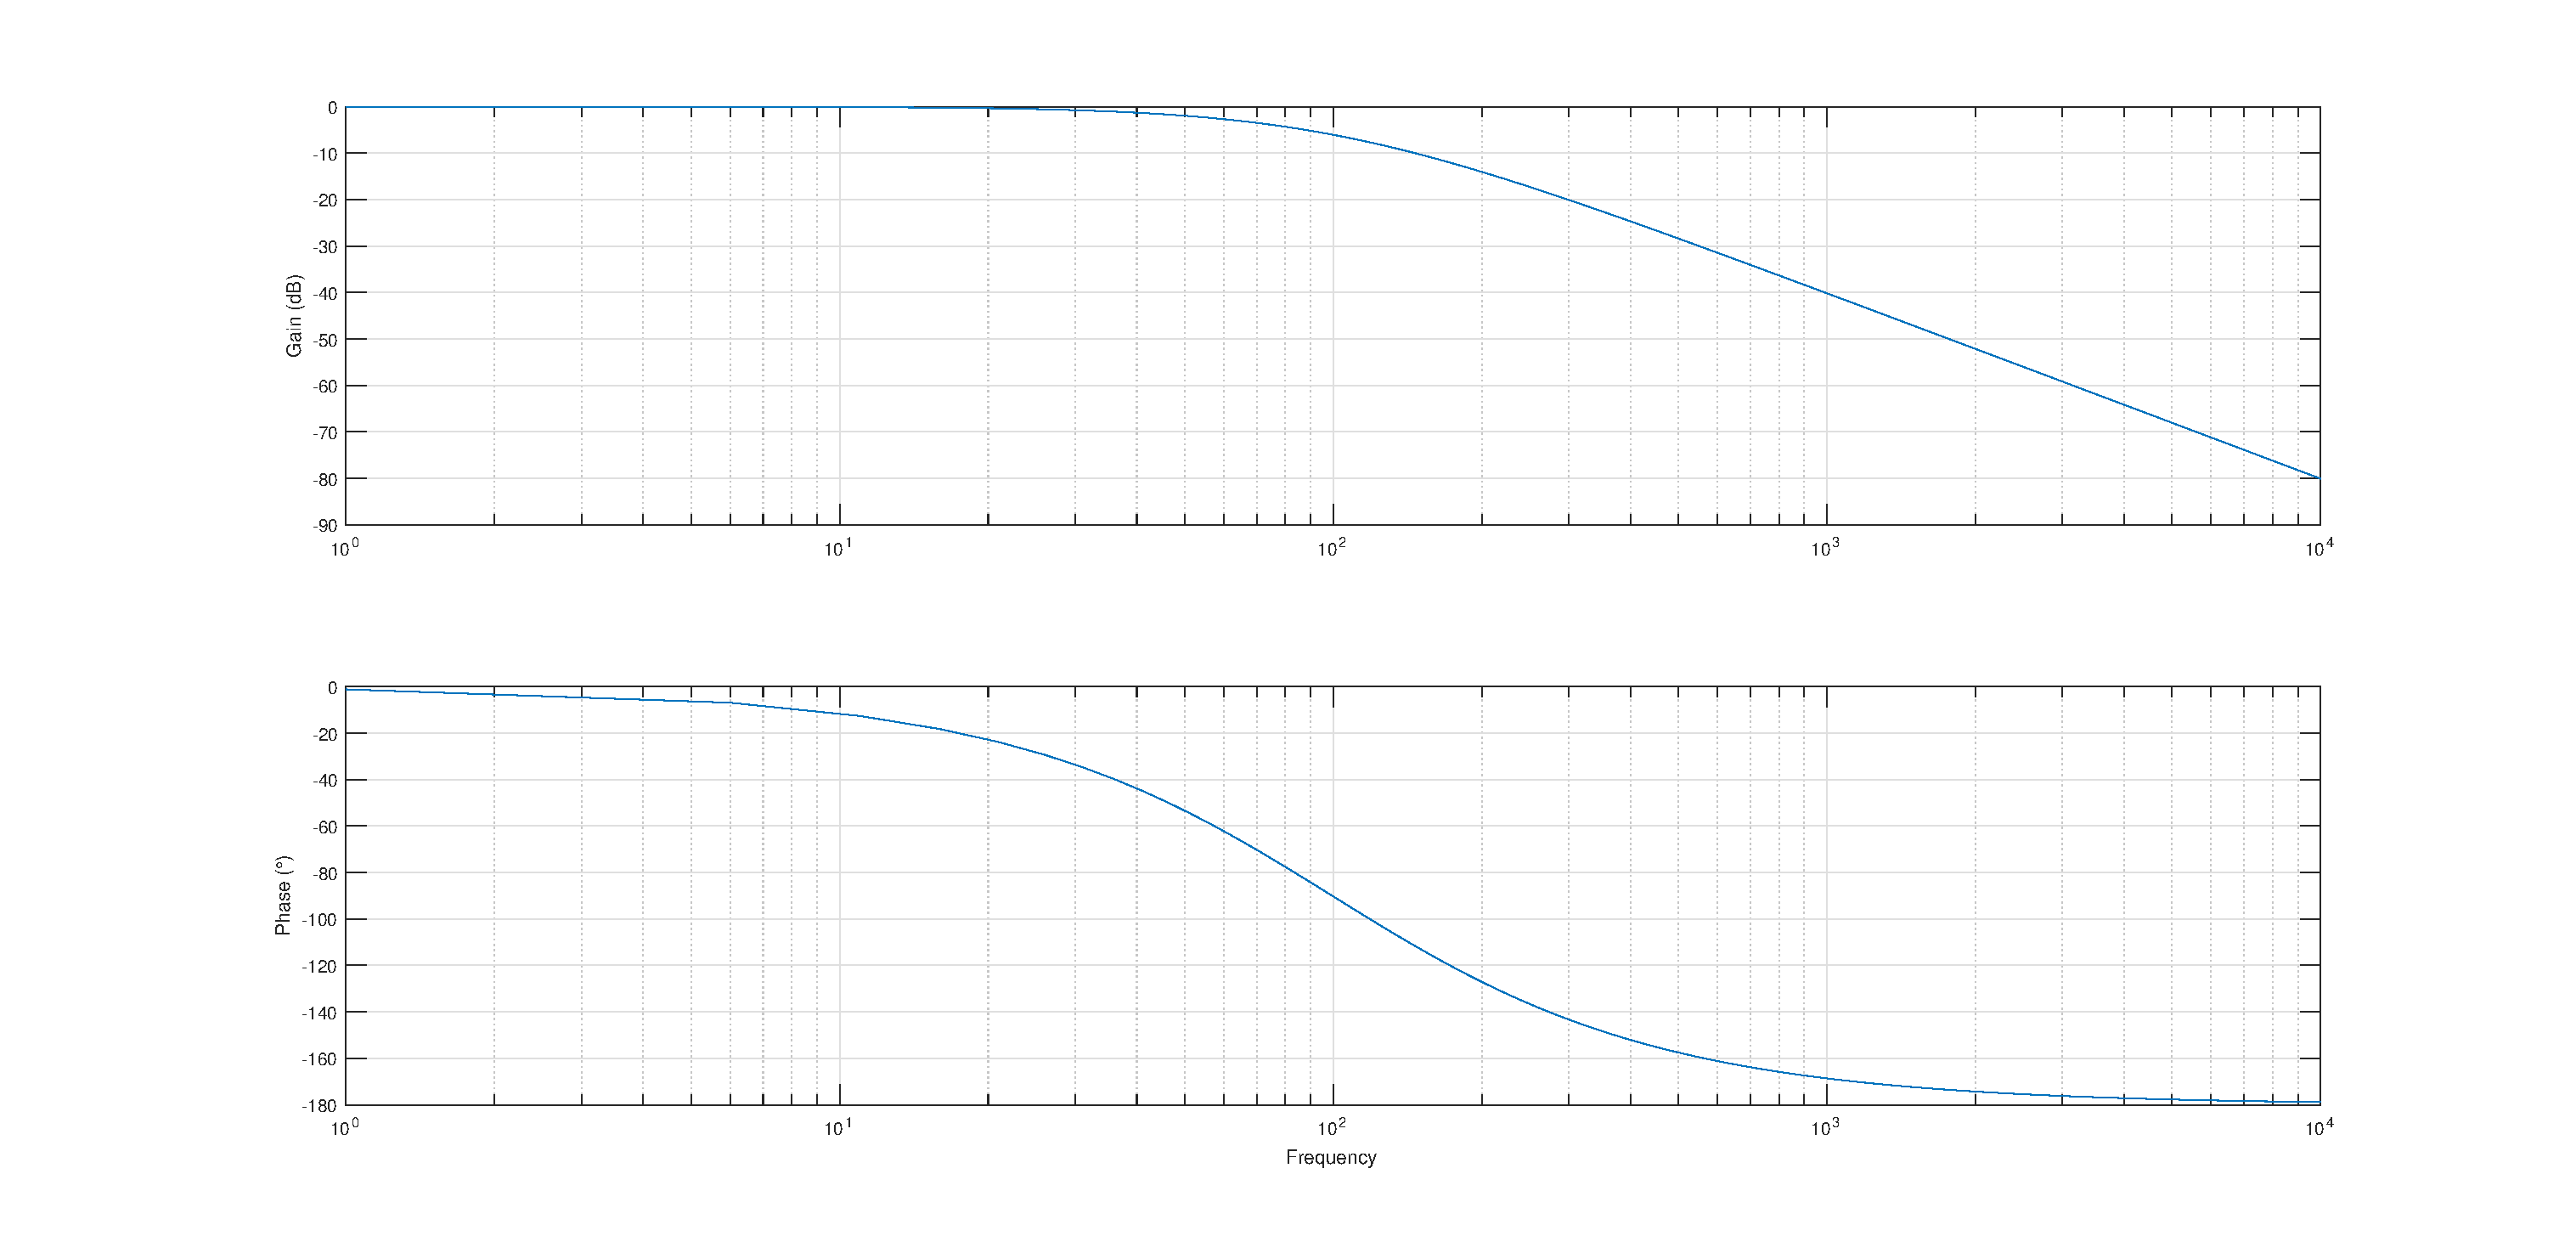
\includegraphics[width=\SchematicWidth]{\Images/Schematic/filter.eps}
    \caption{Bode plot of the filter response}
\end{figure}
\FloatBarrier

The response match our needs, which are quite simple : Remove the potential harmfull noise,
and fast variations that could occur. 

The real circuit on the schematic is based on this one, but with optionnal configurations
jumpers to enable to tune the circuit on board.

This include : 
\begin{itemize}[noitemsep]
    \item   An optionnal voltage divider at the input, to not go above the rail of the OpAmp.
    \item   Optionnals jumpers to bypass the frontend directly to the ADC.
\end{itemize}
\section{RF Antennas}
For this second section, we're going to explore some RF design steps that we done on the PCB,
to draw our antennas for the different modules.

This include a $1.55 \si{\giga\hertz}$ for the GPS signals, and a $2.4 \si{\giga\hertz}$
Bluetooth antenna.

For theses antenna, we've found a nice application note from TI \cite{InvertedF} that
show different examples of RF design for $2.4 \si{\giga\hertz}$  Antenna, and \cite{GNSS}
for the $1.55 \si{\giga\hertz}$ one. Since we don't really know how to properly design an
antenna from scratch, we copied theses design into our schematic and PCB while doing a
little bit of MATLAB simulation on the design to ensure the criterions will be matched.
\section{Power supplies}
Now, let's look a bit deeper on the power supplies, and how they're agenced.
\subsection{Power tree}
To represent the whole power supply organization, we drew a power tree, a schematic that
represent the power supplies.

\begin{figure}[!ht]
    \centering
    \resizebox{\SchematicWidth}{!}{%
        \begin{circuitikz}
            \tikzstyle{every node}=[font=\large]
            \draw [ fill={rgb,255:red,195; green,232; blue,235} ] (-1.25,17.25) rectangle  node {\large Battery 1} (3.75,14.75);
            \draw [ fill={rgb,255:red,195; green,232; blue,235} ] (-1.25,11) rectangle  node {\large Battery 2} (3.75,8.5);
            \draw [ fill={rgb,255:red,218; green,187; blue,217} ] (-1.25,4.75) rectangle  node {\large USB} (3.75,2.25);
            \draw [ fill={rgb,255:red,233; green,235; blue,199} ] (8.75,17.25) rectangle  node {\normalsize 5V buck (2A)} (13.75,14.75);
            \draw [ fill={rgb,255:red,233; green,235; blue,199} ] (8.75,11) rectangle  node {\large 3.3V Buck (200 mA)} (13.75,8.5);
            \draw [ fill={rgb,255:red,236; green,195; blue,195} ] (18.75,17.25) rectangle  node {\large Servo and power circuits} (23.75,14.75);
            \draw [ fill={rgb,255:red,158; green,148; blue,213} ] (18.75,11) rectangle  node {\large Logic IC and analog circuits} (23.75,8.5);
            \draw (6.25,4.75) to[D] (6.25,8.5);
            \draw [short] (3.75,3.5) -- (6.25,3.5);
            \draw [short] (6.25,4.75) -- (6.25,3.5);
            \draw [short] (3.75,9.75) -- (8.75,9.75);
            \draw [short] (6.25,8.5) -- (6.25,9.75);
            \draw [short] (3.75,16) -- (8.75,16);
            \draw [short] (13.75,16) -- (18.75,16);
            \draw [short] (13.75,9.75) -- (18.75,9.75);
            \draw [dashed] (6.25,9.75) -- (6.25,16);
            \node [font=\large] at (5,16.5) {7.4V - 8.2V};
            \node [font=\large] at (5,10.25) {4.3V - 8.2V};
            \node [font=\large] at (15.25,16.5) {5V};
            \node [font=\large] at (15.25,10.25) {3.3V};
            \draw [dashed] (6.25,16) -- (6.25,18.5);
            \draw [dashed] (6.25,18.5) -- (16.25,18.5);
            \draw [dashed] (16.25,18.5) -- (16.25,16);
        \end{circuitikz}
    }%
    \label{fig:power_tree}
    \caption{}
\end{figure}
\FloatBarrier

On this schematic, there two main regulators, that are, in fact buck switching regulators.
But, there's three power sources :
\begin{itemize}[noitemsep]
    \item   Vbus : The 5V that came from the USBC port when the board is plugged on a PC.
    \item   Vbatt : A battery that is charged to power up the MCU and all of the logic
          circuits.
    \item   Vbatt\_pyro : A battery that is charged to power up the servo engines and
          the thruster starter.
\end{itemize}.

As we can see in \ref{fig:power_tree}, we can configure the power supply as we need.
From the three sources, we're able to use a single one by tying both supply together.
And, we can even then supply the whole system with a single USB supply, but at a reduced
voltage. At the opposite, if needed, we can bypass the 5V buck system if we want to
power the servos and the engines with an higher voltage.

Selection is mainly done by jumper, which are big zero ohm resistors.

\subsection{DCDC buck design}
To design theses circuits, we used a reliable tool that may be found online, from
Texas Instruments : \cite{POWERDESIGNER}. We pass them the input conditions, such as
voltage, and the output wanted : voltage and current. The tool output then circuits
than can match the needs, and we need to select one, based on some settings :

\begin{itemize}[noitemsep]
    \item   Space on board
    \item   Cost
    \item   switching frequency
\end{itemize}

Since we didn't require specific criterion on theses aspects, we choose the one that
was the easiest to solder. Then, we import the designed module into the schematic.

\section{Digital part}
For this second part, the digital one we're going to look at the
microcontroller mostly, but also some parts of the whole digital subsystems.
For this part, we mostly got inspired by development kits, such as
\cite{nRF5340DK}. These provide a great example on how to implement some IC on
custom PCBs.

Around the MCU, we added some peripherals IC to fulfill our needs, for examples
:
\begin{itemize}[noitemsep]
    \item An 16 Mb EEPROM, to store flight measurements.
    \item An RGB LED, to indicate status to the user.
\end{itemize}

To ensure the systems are working we sometimes need to modify some elements
from the examples. These changes are always documented in the datsheets of the
components.

Here some examples of things we changed :
\begin{itemize}[noitemsep]
    \item   Change configuration bootstrap to select one mode of the other.
    \item   Configure power supplies needed.
    \item   Configure I2C addresses.
\end{itemize}

\subsection{Pin attribution}
To understand how we assigned to each functions some pins on the MCU, we need
to read the datasheets, mainly the MCU one. It's clearly explained that any
peripheral can be routed to any pins a pin matrix . Nonetheless, there's some
pins that can designed for a specific function. For example, there is two pins
designed for high drain current, where the opposite direction (pull up) is
standard. These pins are designed to handle high speed I2C ! So if we want to
use fast I2C, it's clearly recommended to use them.

The remaining pins were placed arbitrary, because we'll changed that later !
\ref{sec:pin_swap}.

\subsection{Discrete logic}\label{subsec:dis_logic}
On the board, most of the logic is done in software by the MCU. But there's two
hardware functions, related to security features.

These are latching the state of the pin with a DLATCH on the boot of the board,
and an AND gate between the command of the engines and input of the drivers.

This enable us to block the start of engines in hardware rather than by
software only. Thus, if the board is configured as debug mode, it won't be able
to start engines, regardless of the software loaded.


% PCB
% For this section about PCB design, we're going to explain a lot of different
of elements, such as the component placements, the stackup or the layout.

All of theses are going to be explained separately.
\section{PCB Requirements}
Before any layout step, we defined different specifications that need to be followed.

\subsection{PCB Stackup}
Since we used high frequency signals for the Bluetooth and the GPS antenna, as well as
some high speed digital signals (SPI), to ensure their signal integrity as well as a
maximal power transfer, we needed to match the impedances of the tracks to 50 Ohms.

To ensure this criterion will be respected, we needed the selection of a specific stackup.

This stackup took in considerations some parameters :
\begin{itemize}
    \item   Impedance of signals.
    \item   Design rules (width and tolerances).
    \item   Manufacturer abilities
\end{itemize}

We end up on the JLC04101H-3313 stackup, which is generally available for orders. This is a four
layer PCB, because that's much easier to make great routing on it, while maintaining costs low
enough. This one is defined as following :

\begin{table}[!hbt]
    \centering
    \begin{tabular}{| c || c | c | c |}
        \hline
        Layer & Name           & Type        & Thickness             \\
        \hline
        \hline
        -     & Top Overlay    & Overlay     &                       \\
        -     & Top Solder     & Solder Mask & $30.5 \si{\mu\meter}$ \\
        L1    & Top            & Copper      & $35 \si{\mu\meter}$   \\
        -     & Dielectric 2   & Prepreg     & $99.4 \si{\mu\meter}$ \\
        L2    & GND1           & Copper      & $15.2 \si{\mu\meter}$ \\
        -     & Dielectric 1   & Dielectric  & $700 \si{\mu\meter}$  \\
        L3    & INT2           & Copper      & $15.2 \si{\mu\meter}$ \\
        -     & Dielectric 2   & Prepreg     & $99.4 \si{\mu\meter}$ \\
        L4    & Bottom         & Copper      & $35 \si{\mu\meter}$   \\
        -     & Bottom Solder  & Solder Mask & $30.5 \si{\mu\meter}$ \\
        -     & Bottom Overlay & Overlay     &                       \\
        \hline
    \end{tabular}
    \caption{JLC04101H-3313 PCB Stackup}
    \label{tab:stackup}
\end{table}
\FloatBarrier

On this stackup, we defined for each layer a precise role.
The top (L1) and bottom (L4) layers are used for general trace routings, where the second
layer (L2) is used as a ground plane, that is used as reference for impedance matched
signals, and to provide shielding between top and bottom layers.

Thus, high speed signals are routed on top layer (L1) to be nearer of the reference plane, and
where return current can be the closed to the forward path.
On the opposite side, there's the slower signals, that won't suffer from a further ground plane.

The last layer, (L3), is a plane that was at first designed to be another ground plane, with the
power delivery network (PDN) on it, routed with wide traces. Since it was too difficult to
properly route the signal out of the microcontroller, we're forced to add some signals traces too.
To ensure signal integrity, as well as the bottom (L4) layer, we didn't routed fast signals here.

\subsection{Board Shape}
The next parameter to be accounted before starting the layout is the board shape. Since
we're in a size constrained situation, we defined the board shape when designing the
mechanical support.

This gave us a board shape like that :

\begin{figure}
    \centering
    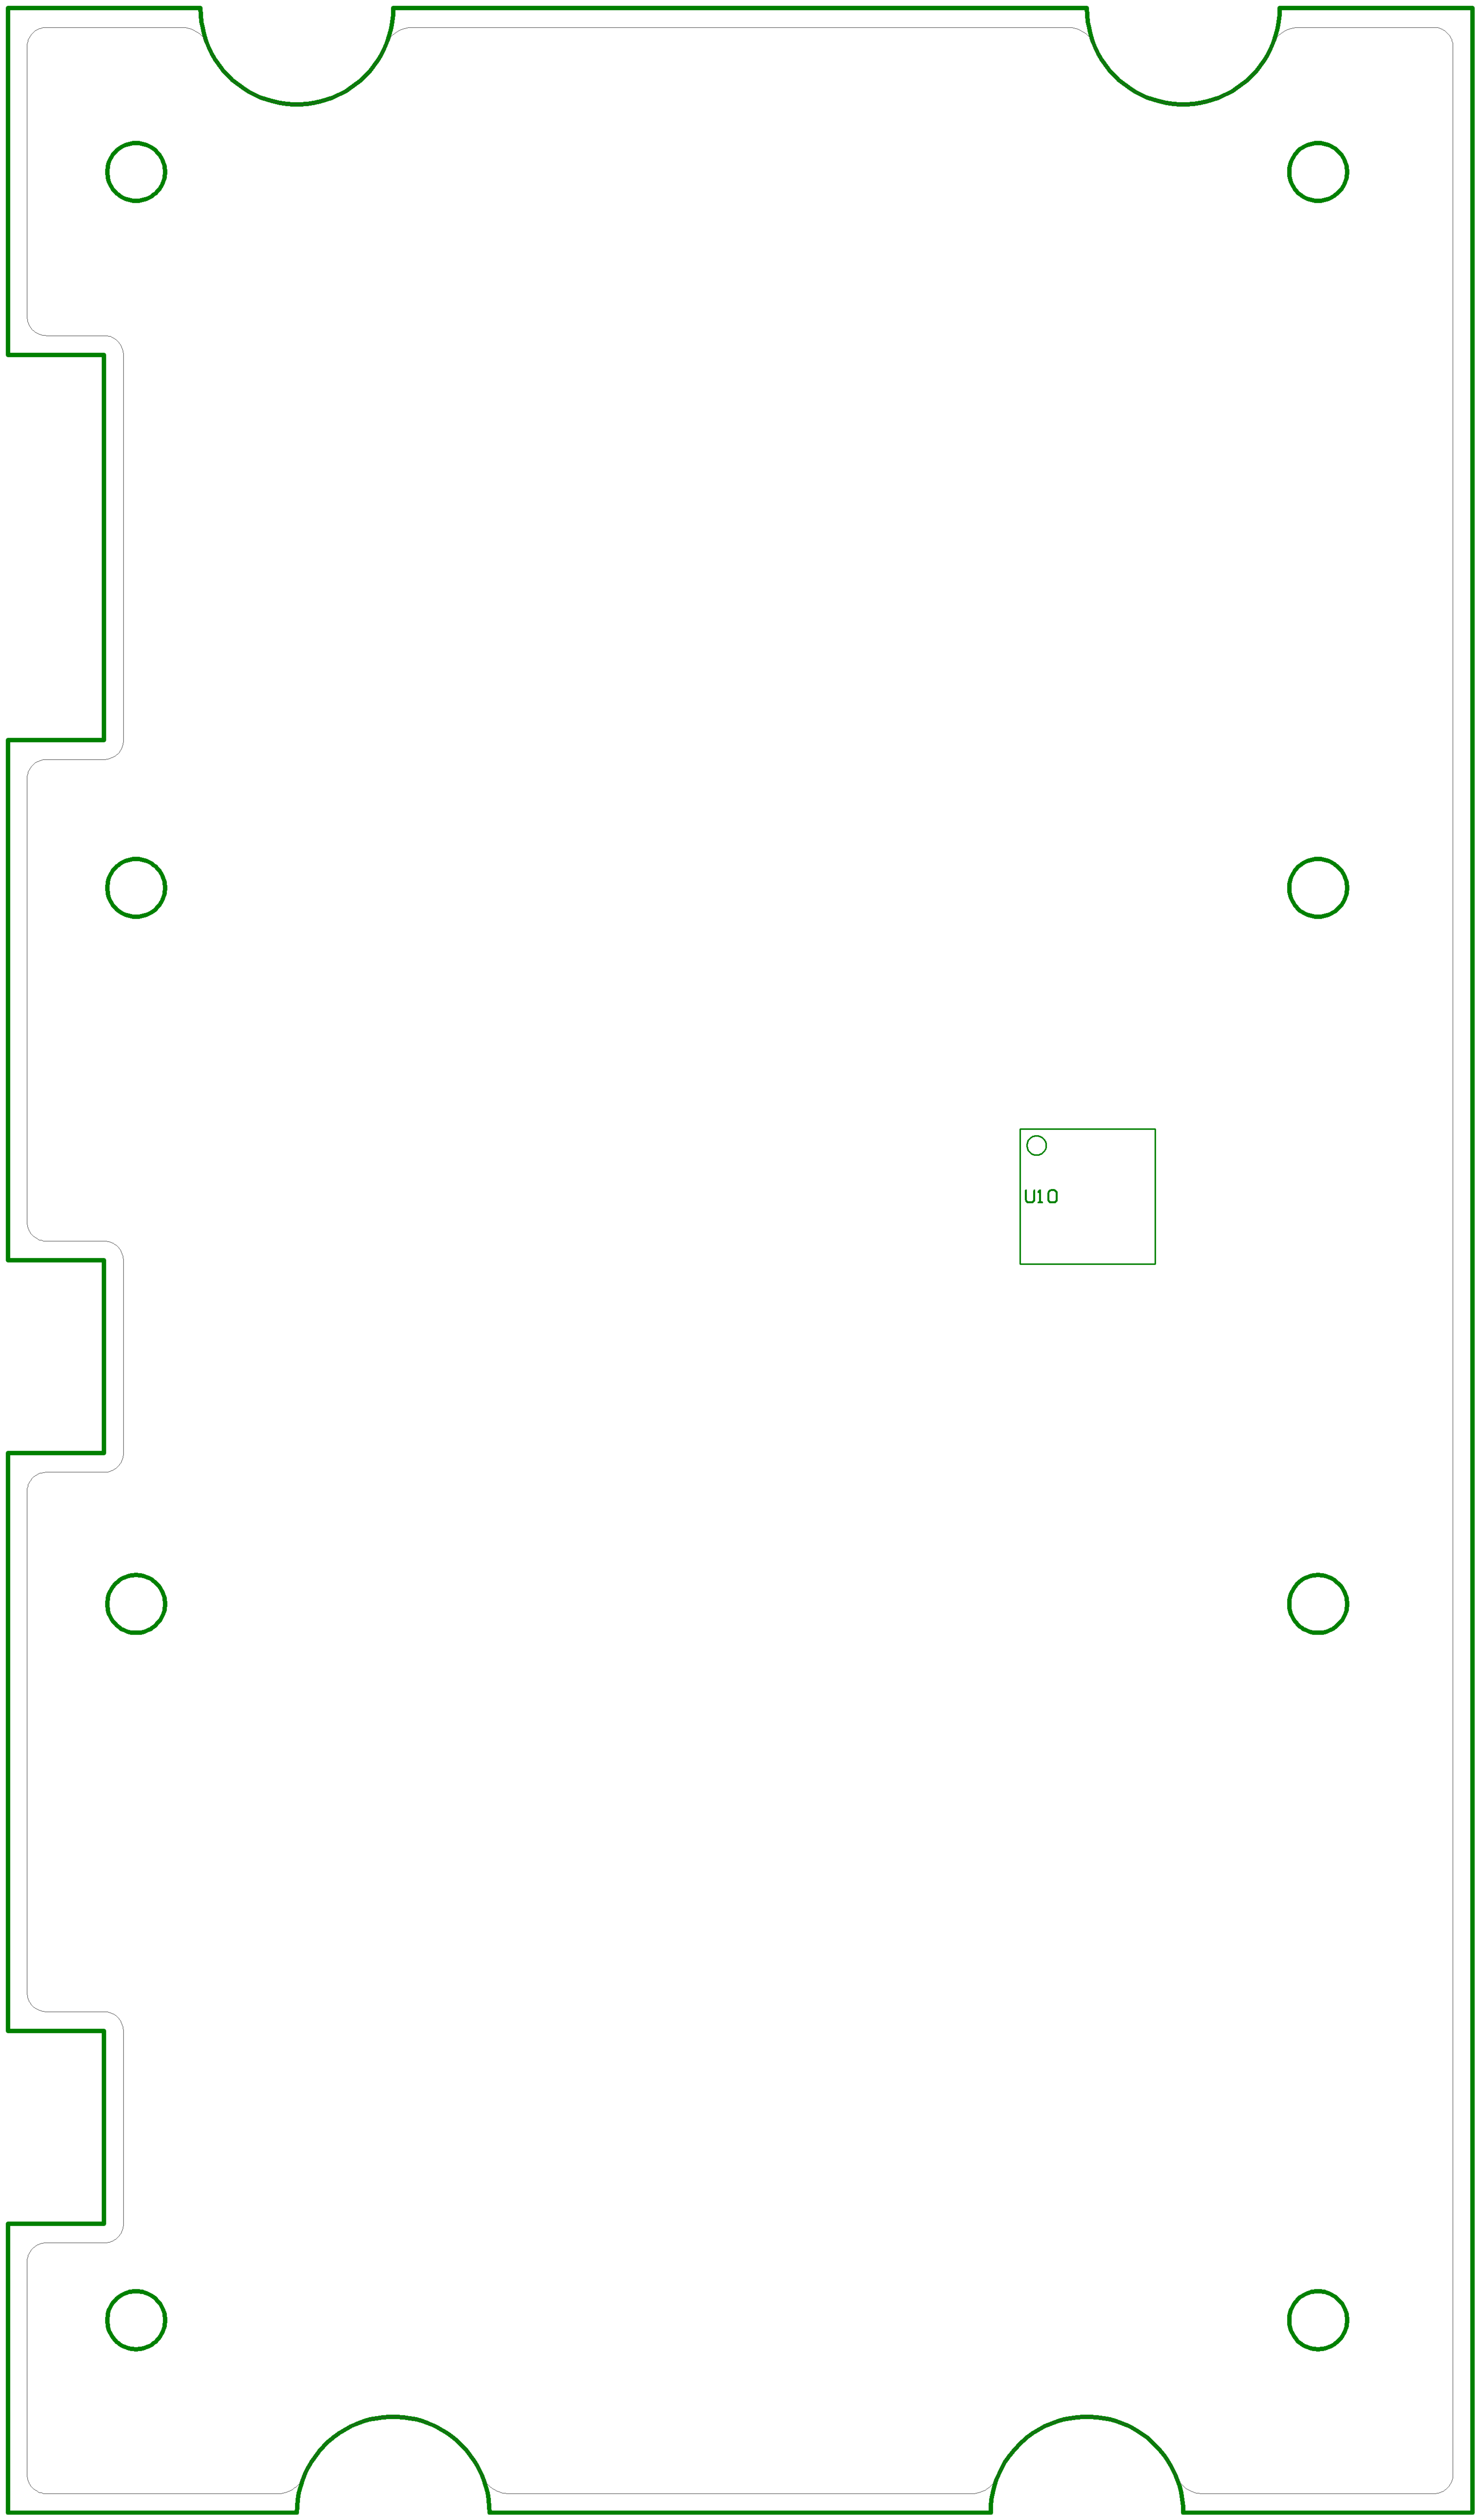
\includegraphics[width=\SmallSchematicWidth]{\Images/PCB/shape.eps}
    \caption{Board outlines}\label{img:board_shape}
\end{figure}

In green, and with right angles, there the exported shape from the mechanical conception.
We defined a bit smaller board shape than that, to ensure that the manufacturing tolerances
wont cause any issues, and to add some margin. This final board shape \ref{img:board_shape}
is not clearly visible on the image, as it's drawn in grey and on a thin line.

There's a lot of mechanical support, by both screws and cuts to ensure the board can't be
mounted backward. This is required to ensure the positing system has always the same
reference position.

And, to finish, there some cutouts on the left side, to let more space for wirings. Thus, we
can easily make wires runs from the engines to the board without stressing them.

\FloatBarrier

\subsection{Floorplan}
From all of theses settings, we can establish a first floorplan. As there is some cutouts for
wires on the board, the position of some connectors / soldering pads need to be defined, to
ensure the wire won't need to cross the board !
But there a lot of others elements with a defined position, theses includes :

\begin{itemize}[noitemsep]
    \item   Antennas and related ICs / passives (need to be closest to the source, with excellent
          grounding)
    \item   Position of the accelerometers and IMU (Shall be placed near to the center of the board
          to prevent from rotationals events)
    \item   Position of the screws (Defined by the support)
\end{itemize}
\section{PCB Layout}
Now, we can start the layout process, in this order :

\begin{itemize}
    \item   Place the remaining components on the board
    \item   Route sensibles tracks.
    \item   Route the remaining tracks
\end{itemize}

\subsection{Component placement}
Our board is quite big for the components we needed to place. Thus, there is some empty spaces,
which is not a bad thing.

This also mean that the placement of passives (which are, for most in the package size 0603)
easier, since circuits are physically distants from others.

For each circuits, we always start with the decoupling capacitors, that need to be carrefully
placed near each power pins of the circuits. Then, we place the remaining passives that can
be placed farther from the chip, for example pull up resistors.

This whole process was iterated two times. On the first pass, we globally place the components,
within 2 or 3 mm of their final position. Once the whole board was done, we've got a first idea
of what the board was going to look, but there were a lot of smaller optimization that could be
done. That's the goal of the second pass, we replace every component to a place that can be easier
to route, aligned with the grid.

\subsection{Pin swapping}
For the next step, we configured the "pin swapping" function on the schematic, to enable some pins
to be swapped. This is possible due to the architecture of most recent microcontrollers, where all
of the functions goes trough a pin matrix to assign to a pin, regardless of the peripheral. This
gave us freedom on the crossing that can be deleted with it \footnote{
    This pin swapping method caused us some harm, because of an undoumented limitations : A
    peripheral can't use, at the same time multiples pins from different ports. This required
    us to re-route some part of the PCB.
}.
We created thus four groups of pins :
\begin{itemize}
    \item   A digital group on the port where the function is pinned to the port 0.
    \item   Another digital group, for the port 1.
    \item   An analog input group.
    \item   A global group, for independant pins that can be used on any port.
\end{itemize}

Then, the ECAD tool enable us to automatically perform pin swapping to globally optimize the pins.
Then, when routing, we can perform some precisions pin swaps if it make the layout easier.

\subsection{Layout}
When routing the connections, we've always got in mind the signal integrity issues than can come
from mistakes at this point.
Thus, we make sure that any fast signal \footnote{
    In fast, near every signal on the board can be qualified as fast, due to their rising and falling
    edges. Nonetheless, for signals that enable or disable functions once in the flight, we assumed
    that their behavior when switching aren't going to perturb the overall execution.
} is routed on top layers, or, by default with a ground plane near it.

For every signals, if they need to "cross" a signal, on another layer, we ensured the crossing to be
at a 90 degrees to reduce the crosstalk between them. In the same manner, we ensured that tracks that
are sensible won't couple inductively. This is done by separating them with enough space \footnote{A
    General rule of thumb is the 3W rule. Track center to the next center, there shall be 3 times the
    width.}

For every track, we needed to route with a correct width, to ensure the current carying capacity will
large enough. Thus, for power tracks such as the 5V rail for the servo engines, or the engines starter,
we respectively used 1.5mm wide tracks. For the 3.3V rail, that power up all of the logic, the current
is smaller, a 1mm wide track is more than enough.

To be added, where there where a lot of pads of the same net to connect together, we used planes rather
than tracks. This greatly increase the current capacity of this area, for a null cost.

To place tracks in a cleaner way, we divide by two the grid, enabling us the ability to pass exactly
in the middle of two pins, to arrive right to the center of a pad.

All of this work is shown on the images below, where we can see each layer, individually, with the
standard Altium color code.

\begin{figure}[!hbt]
    \centering
    \begin{minipage}[c]{\SmallSchematicWidth}
        \centering
        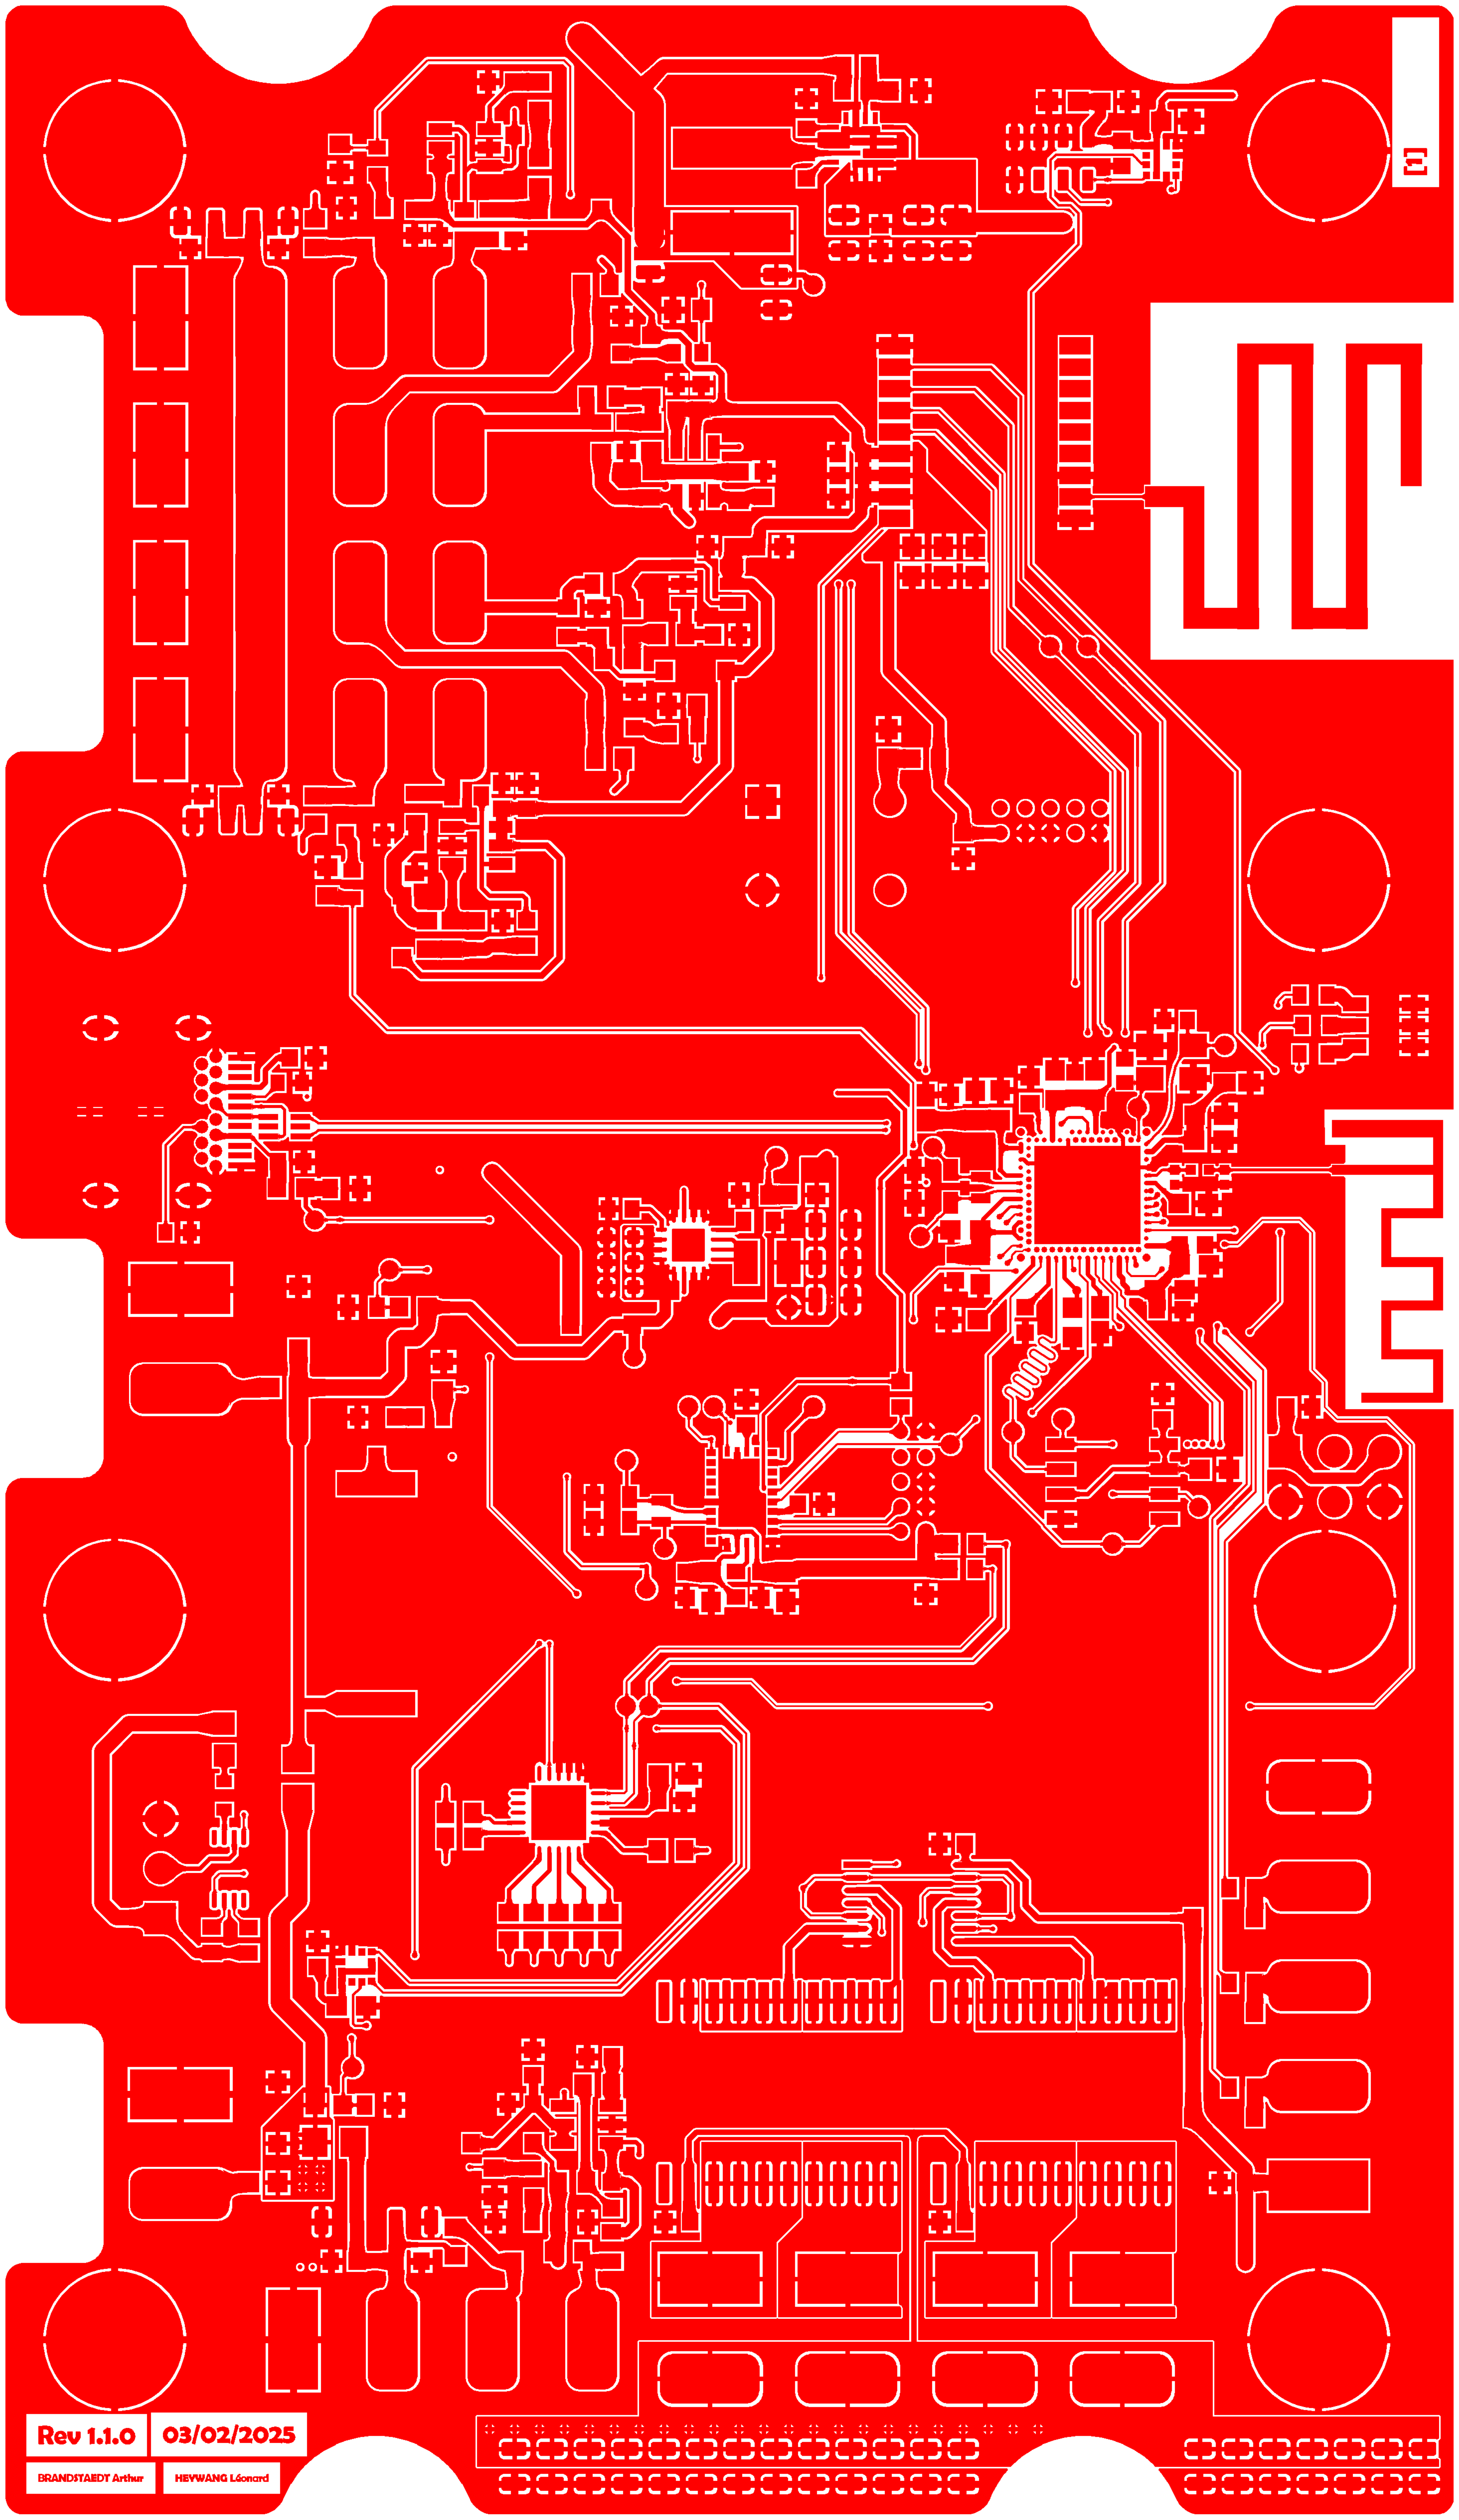
\includegraphics[width=\textwidth]{\Images/PCB/top.eps}
        \caption*{Copper layer (L1)}
    \end{minipage}%
    \hfill%
    \begin{minipage}[c]{\SmallSchematicWidth}
        \centering
        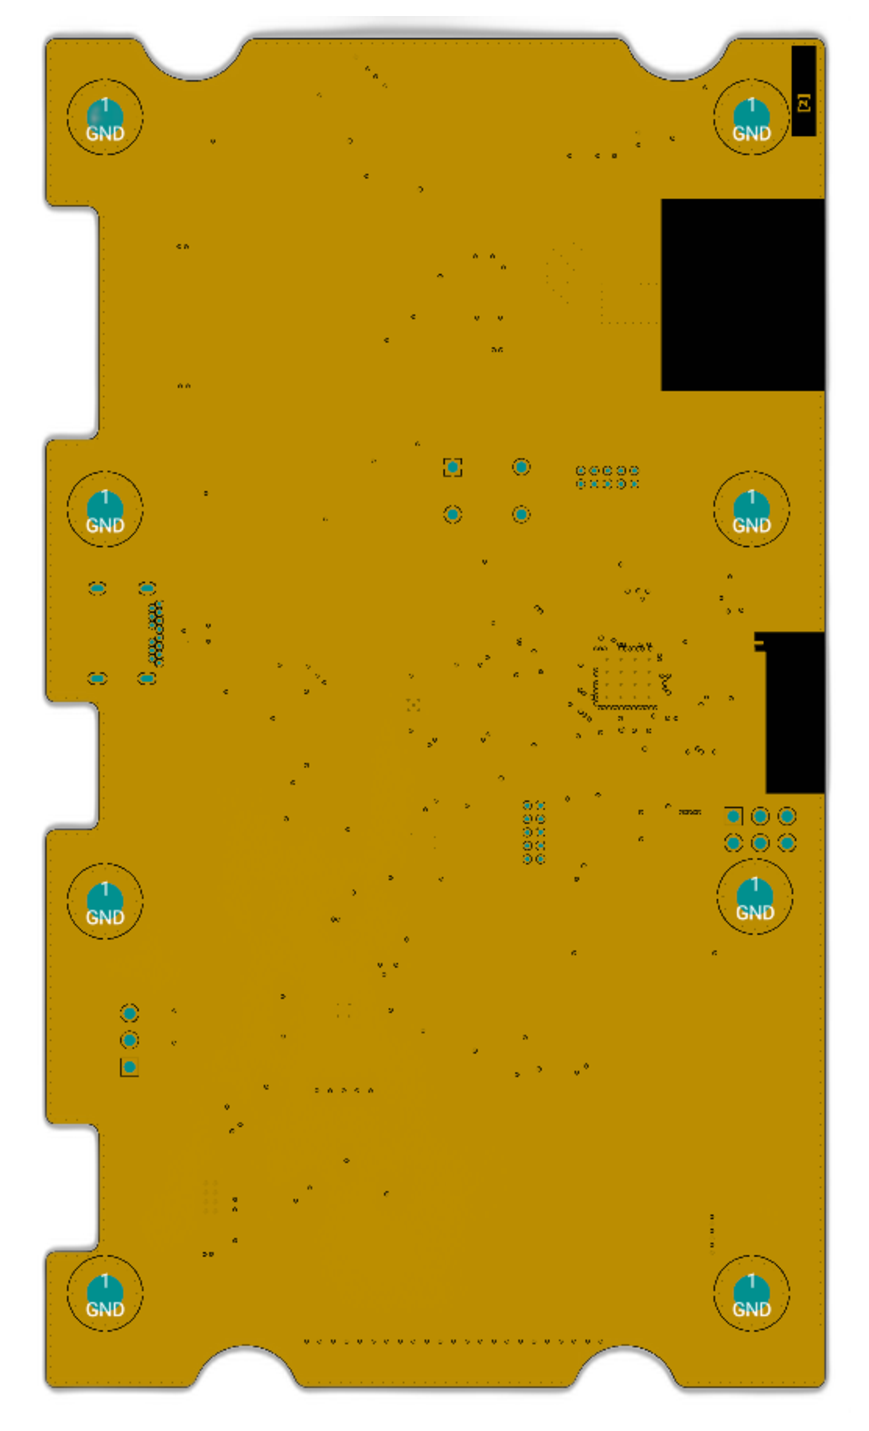
\includegraphics[width=\textwidth]{\Images/PCB/int1.eps}
        \caption*{Copper layer (L2)}
    \end{minipage}%
    \hfill%
    \begin{minipage}[c]{\SmallSchematicWidth}
        \centering
        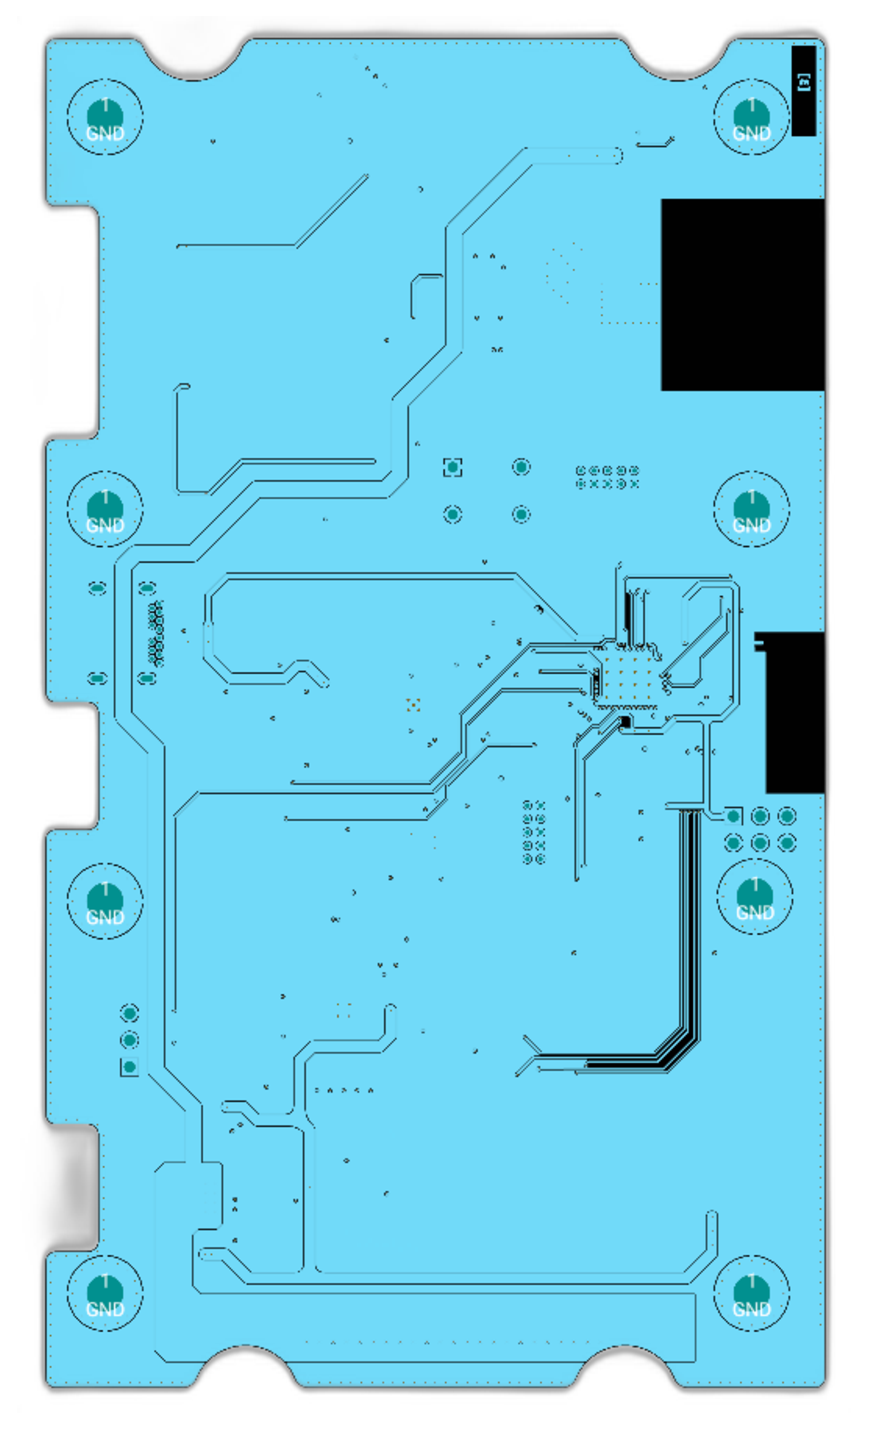
\includegraphics[width=\textwidth]{\Images/PCB/int2.eps}
        \caption*{Copper layer (L3)}
    \end{minipage}%
    \hfill%
    \begin{minipage}[c]{\SmallSchematicWidth}
        \centering
        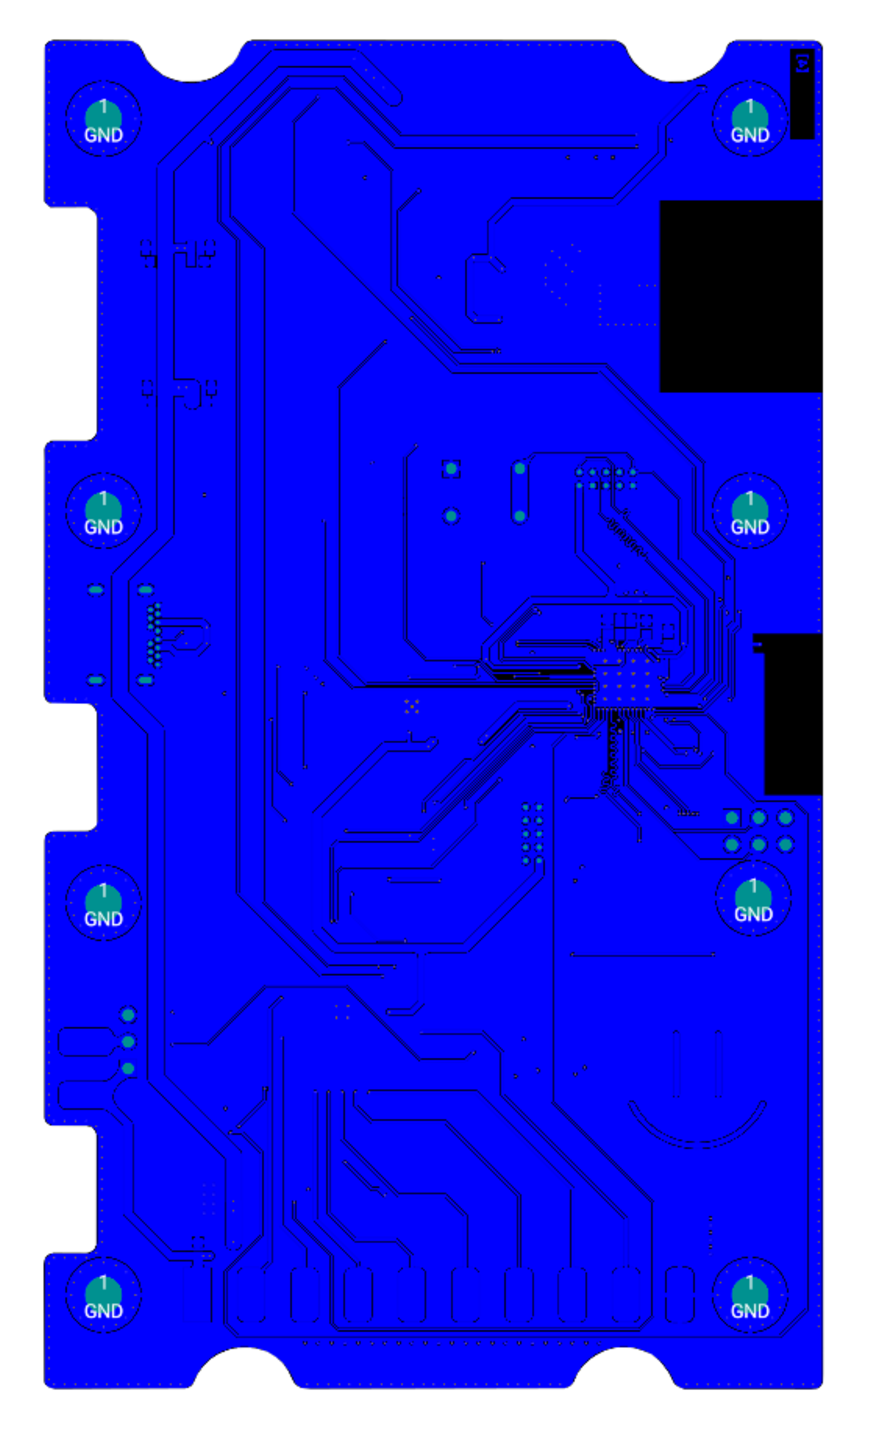
\includegraphics[width=\textwidth]{\Images/PCB/bot.eps}
        \caption*{Copper layer (L4)}
    \end{minipage}
    \label{img:layout}
    \caption{Copper layers on the PCB}
\end{figure}
\FloatBarrier

As explained before, we can cleary see that the first (L1) and last (L4) layers
are the most filled with tracks. The second layer (L2) is effectively empty of
traces, to let the space for a whole ground plane, and, on the last layer there
is the mix of both.

Once the layout was finished, we did some more steps to make the PCB cleaner :

\begin{itemize}
    \item
\end{itemize}

% Assembly
\section{Soldering}\label{sec:assembly}
For the last part of the electronic chapter, we're going to talk about
assembly of the board.

The board use complex components, where the packages are BGA, aQFN...
All of the pitch are in the $0.5 \si{\mu\meter}$ range, thus, it's
evident that it won't be possible to solder it with an iron.

To solder theses components, we used a technic based on industrial
processes, which consists of different steps :

\begin{itemize}
    \item   Apply some solder pastes on the pads.
    \item   Place the ICs and passives on their spots.
    \item   Heat the whole board, to make the solder paste melt.
    \item   Let the board cool down.
\end{itemize}

Solder paste is a mix of tin and flux. It's used to create precision
soldering, since it's much easier to get the rigth volume of tin on a
point.

\subsection{Solder paste application}
First, we need to apply solder pastes. The smallest pads are round,
$200 \si{\mu\meter}$ in diameter, and $500 \si{\mu\meter}$ far from the
other.

It's then impossible to place solder paste by hand on this pads.

That's why we used a stencil, that we place over the board, and fix in
place with different tools. Then, we apply some paste on this stencil, and
we spread it on the board with something rigid enough.

This will fill the stencil holes with the right volume of paste, and, if
correctly placed, right over the pads. Once finished, we remove the stencil,
and there shall be right enough paste, we it needs. \footnote{
    Since the paste is about half flux, getting a bit of paste where it shouldn't
    isn't generally an issue. And, with surface tension of melted tin, it will
    generally flow to the contact without issues.
}

\subsection{Placing the SMT}
Once we're satisfied with the paste application, we can start to place components.

This step can be quite long, since it require a lot of application, and concentration.
Hopefully, there is some tools to make it easier, such as Altium assembly assistant,
which will prompt us which reference goes where, and in which orientation.

This make the placement much faster and right.

Once all components are placed, we inspect them. They need to be precisely placed
for all of them\footnote{
    When the board is hot enough, again, the surface tensions of the melted tin will
    tend to place the IC by themselves. Imprecisions can be corrected here, for a
    maximum of half the distance between two pads.
}. In our board, there is 286 of them !

\subsection{Heating}
For the final part, we need to heat the board. There is multiple solutions here,
we can do it on a specific furnace on the FabLab, or, with an hotplate at home.

We tried the second solution for the first board. This plate is going to heat to
$250 \si{\degree}$, heating the whole board in the same time. All of the paste will
melt in the "same" time, and thus all of the solder will be done in one time.

Once finished, we remove the board carrefully of the heating plate, and wait for it
to cool.

All of the process is in photo right below :

\begin{figure}[!hbt]
    \centering
    \begin{minipage}[c]{\SmallSchematicWidth}
        \centering
        \includegraphics[width=\textwidth]{\Images/assembly/assembly_STENCIL.eps}
        \caption*{Stencil placement}
    \end{minipage}%
    \hfill%
    \begin{minipage}[c]{\SmallSchematicWidth}
        \centering
        \includegraphics[width=\textwidth]{\Images/assembly/assembly_PASTE.eps}
        \caption*{Solder paste applied}
    \end{minipage}%
    \hfill%
    \begin{minipage}[c]{\SmallSchematicWidth}
        \centering
        \includegraphics[width=\textwidth]{\Images/assembly/assembly_SMT.eps}
        \caption*{PCB with the SMT placed}
    \end{minipage}%
    \hfill%
    \begin{minipage}[c]{\SmallSchematicWidth}
        \centering
        \includegraphics[width=\textwidth]{\Images/assembly/assembly_HOTPLATE.eps}
        \caption*{PCB on the heating surface}
    \end{minipage}
    \label{img:assembly}
    \caption{assembly process}
\end{figure}
\FloatBarrier

After that whole process, we need to add the few trough hole components, manually.
This is quite fast, since there is not a lot of them.
\section{Testing and defaults}\label{sec:defaults}
Once the board is finished, we need to test it. And, in our case, the $3.3
    \si{\volt}$ and the GND were in short-circuit. Most of the nets where fine.

To search for the location of the default, we used an electronic magnifying
glass. We found these defaults :

\begin{figure}[!hbt]
    \centering
    \begin{minipage}[c]{0.32\textwidth}
        \centering
        \includegraphics[width=\textwidth]{\Images/assembly/default_SOLDER.eps}
        \caption*{Too much solder}
    \end{minipage}%
    \hfill%
    \begin{minipage}[c]{0.32\textwidth}
        \centering
        \includegraphics[width=\textwidth]{\Images/assembly/default_SOIC.eps}
        \caption*{Lack of heat n1}
    \end{minipage}%
    \hfill%
    \begin{minipage}[c]{0.32\textwidth}
        \centering
        \includegraphics[width=\textwidth]{\Images/assembly/default_CAP.eps}
        \caption*{Lack of heat n2}
    \end{minipage}%
    \label{img:defaults}
    \caption{assembly defaults}
\end{figure}
\FloatBarrier

\subsection{Hand soldering default}
The first default came from the use, when soldering with hand some of the
capacitor on the back side.

At first, the solder was looking quite good, but, under magnification, we found
that some contacts where touching between them.

This kind of issues are easily corrected by removing the excess solder, with,
for example a solder wick.

\subsection{Heating defaults}
The two last defaults are a bit harder to patch. They come from a lack of heat
on the board, which didn't make fully melted the solder paste. Thus, there is
some tin balls on multiple places of the PCB.

This is probably the source of our short circuits, because the nets that are in
short-circuits are always side by side under the microcontroller.

This kind of defaults can be patched by reheating the board, with enough flux.

\subsection{Defaults removal}
When reheating the board, the defaults didn't disapeared, leaving us with a
defective board.

We then soldered two anothers boards, with a slightly different technique to
apply solder paste. This method gave us greater results, and we end up with two
working boards.
